
\documentclass[18pt]{beamer}
\usepackage{templates/beamerthemekit}
\usepackage[export]{adjustbox}
\usepackage{tikz}
\usepackage{bbm}
\setbeamercovered{invisible}

\usepackage{latexsym,amsmath,amssymb,mathtools,textcomp}
% \usepackage{templates/beamerthemekitwide}

% \titlelogo{mylogo}
% \usepackage{templates/tikzkit}
% \usepackage{templates/tikzuml}
% \titleimage{myimage}


\titlelogo{myimage}


\title[Bachelor's Thesis]{Creating and Evaluating \\Stochastic Regression Models \\on the Basis of Heterogeneous Sensor Networks}
\subtitle{Bachelors Thesis, Supervisors  - Dr. Johannes Riesterer, Dr. Sebastian Lerch}
\author{Stanislav Arnaudov}
\date{7. November 2018}

\institute{TECO - Das Telecooperation Office}
\usepackage[citestyle=authoryear,bibstyle=numeric,hyperref,backend=biber]{biblatex}
\addbibresource{templates/example.bib}
\bibhang1em

\begin{document} 

% \selectlanguage{english}
\selectlanguage{ngerman}


\begin{frame}
  \titlepage
\end{frame}

\begin{frame}
  \frametitle{Motivation}  
  Given is a heterogeneous network of sensors -- the network contains ``good'' \textbf{and} ``bad'' sensors.\\
  \begin{itemize}
  \item good -- calibrated and high precision of the measurements 
  \item bad -- uncalibrated and low precision of the measurements
  \end{itemize}
  Interesting Questions:
  \begin{itemize}
  \item Can we use the bad sensors in order to predict the values of the good ones?
  \item Can we identify the weak parts of the network?
  \end{itemize}
  Our approach to the problems:
  \begin{itemize}
  \item Use of stochastic regression models.
  \item Formal evaluation of the models through the use of proper scoring rules, verification rank histograms and predictive performance checks.
  \item Analyzing the relevance of each predictor for the final prediction through the use of a feature importance technique.
  \end{itemize}
\end{frame}

\begin{frame}
  \frametitle{Data}
  \begin{itemize}
  \item Heterogeneous Network of air pollution sensors in Stuttgart.\\
    \begin{itemize}
    \item LU-BW (\textit{Landesanstalt für Umwelt, Messungen und Naturschutz Baden-Württemberg}) - \textbf{3 Sensors} of high quality.
      \begin{itemize}
      \item Station names: SBC, SNTR, \textcolor{red}{SAKP}
      \end{itemize}
    \item \textit{luftdaten.info} -- Public data from cheap DIY sensors.
    \end{itemize}
  \item Considered period: the year of 2018.
  \item Challenges:
    \begin{itemize}
    \item Noisy data.
    \item Holes in the data.
    \item Station SAKP provides air pollution values only for the last four months of the considered year.
    \item The DIY sensors provide values for each minute of the day, the LUBW sensors - for thirty-minute
intervals
    \end{itemize}
  \end{itemize}
\end{frame}

\begin{frame}
  \frametitle{General View}
  \vspace{-0.2in}
  \begin{center}
    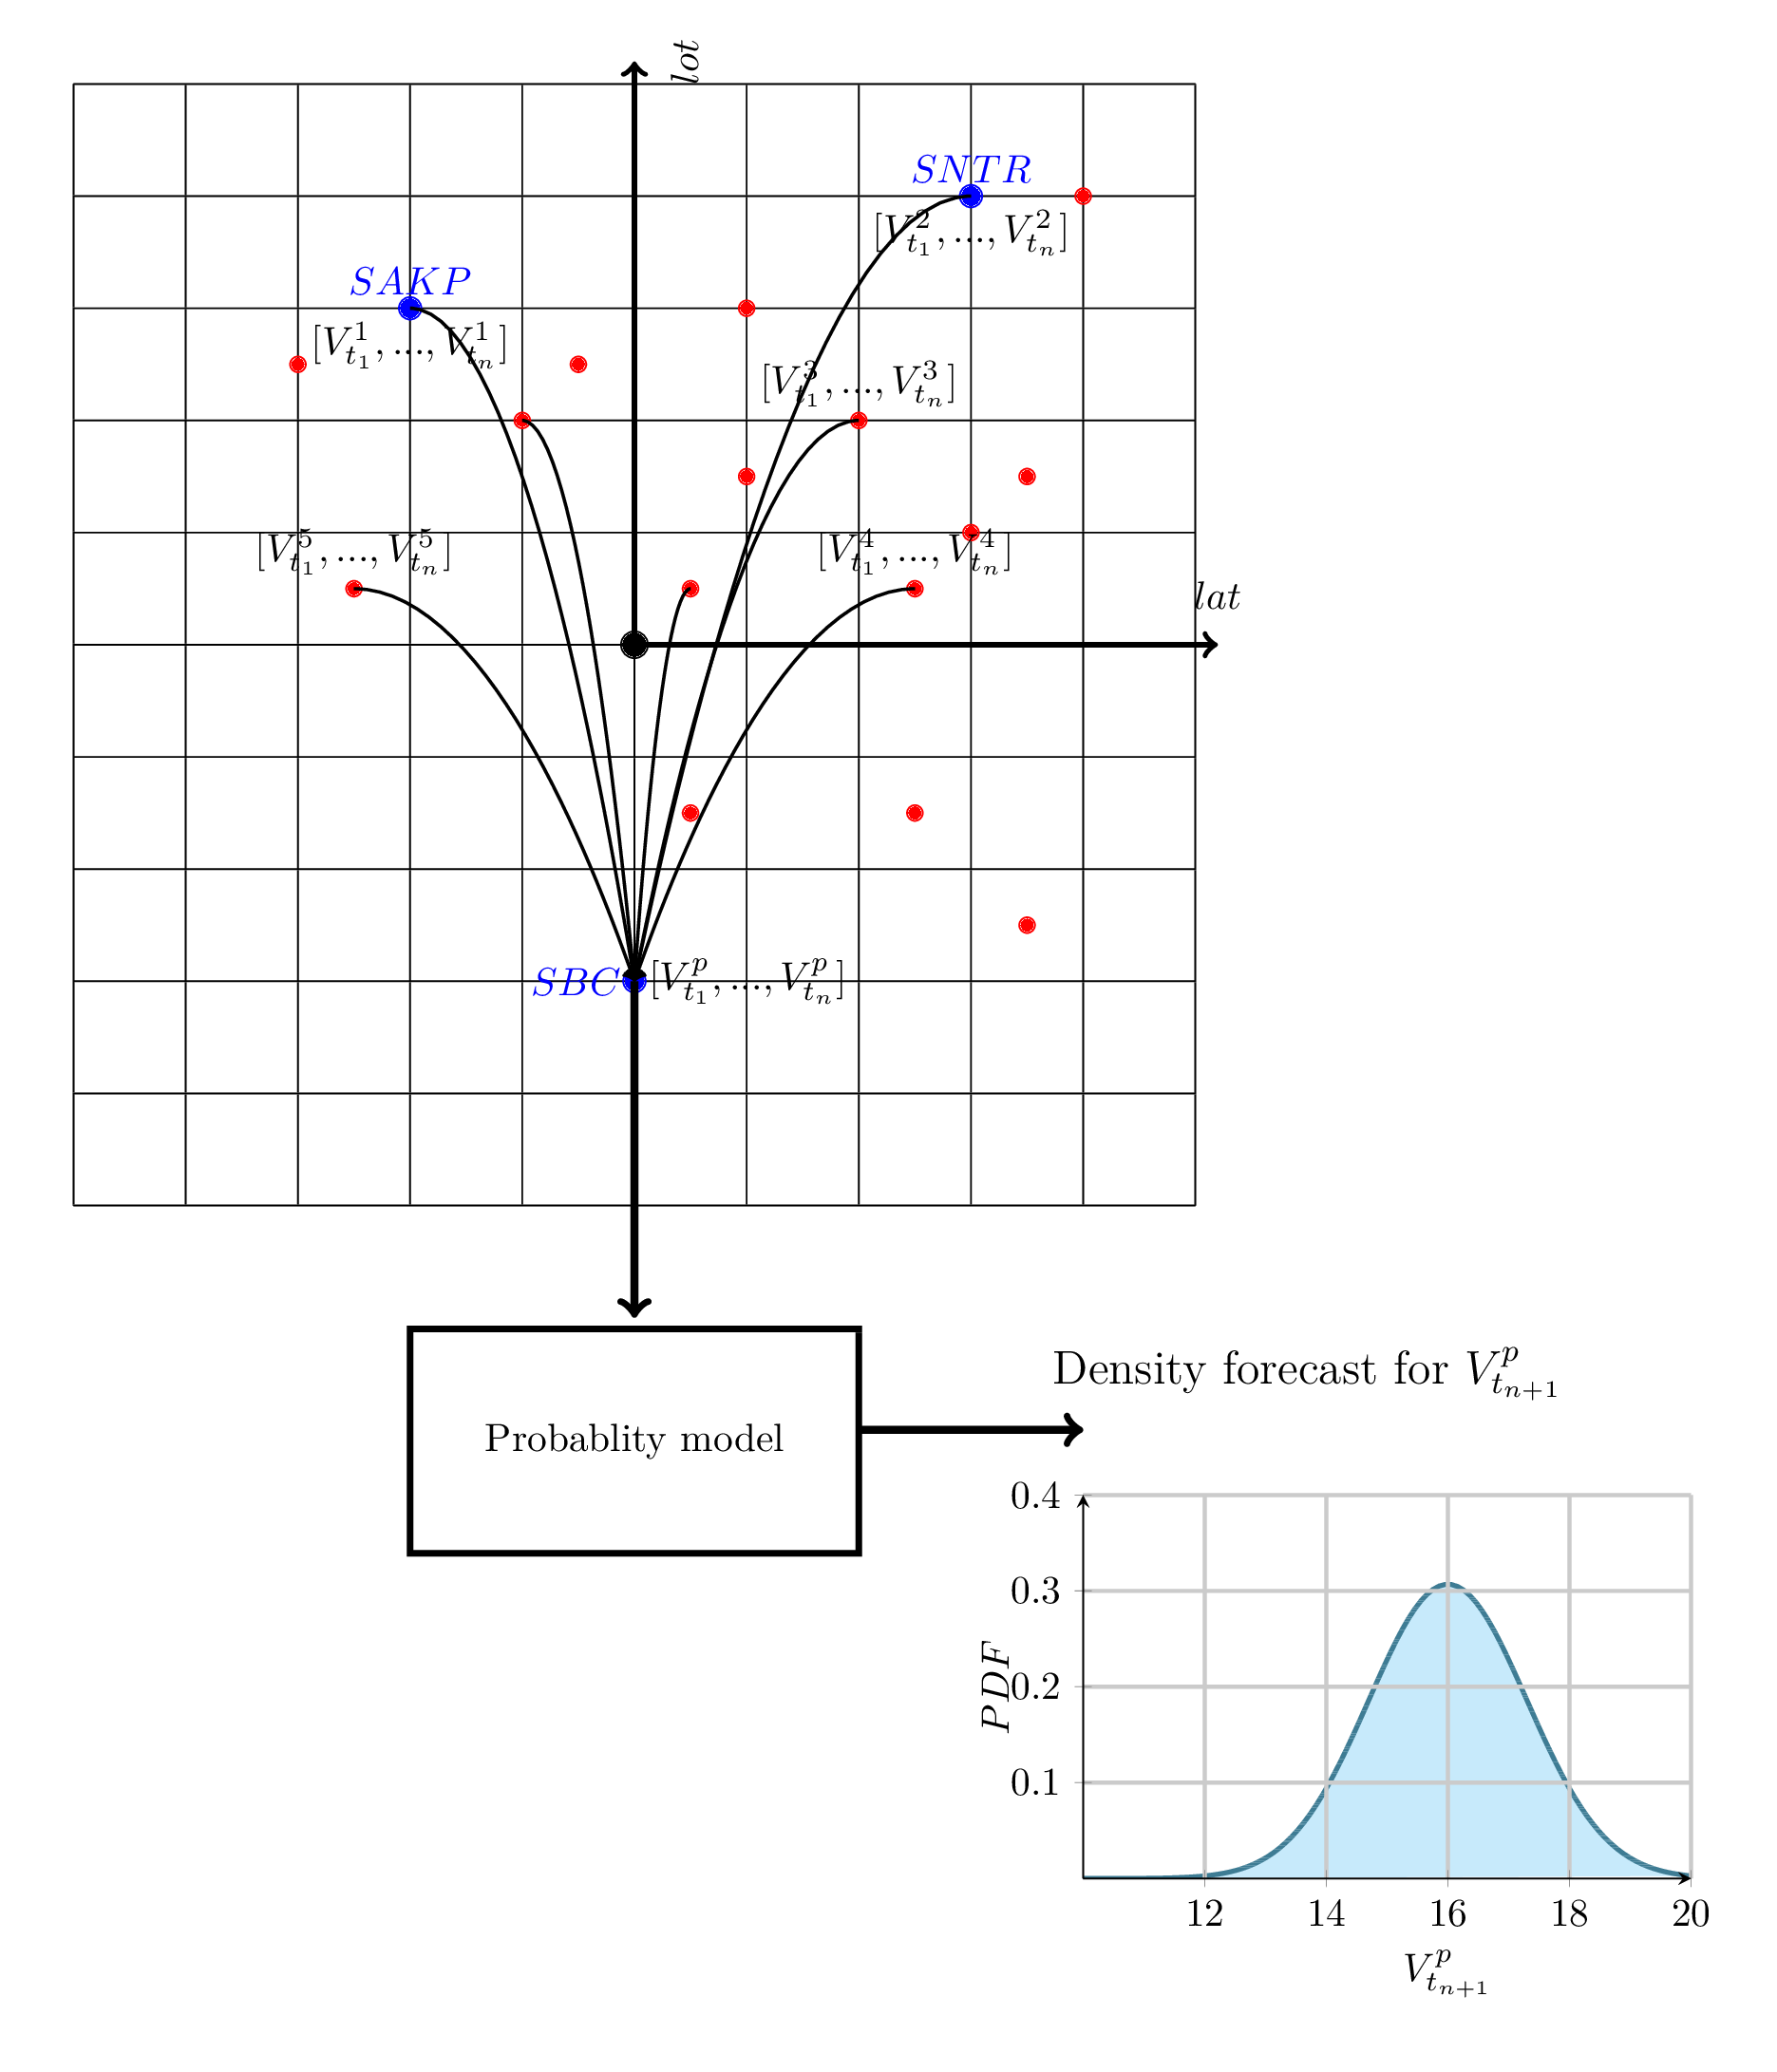
\includegraphics[scale=0.10]{images/general_system}
  \end{center}
\end{frame}

\begin{frame}
  \frametitle{Goals and not goals}
  Goals:
  \begin{itemize}
  \item Investigate how the considered models perform on the data.
  \item Show that the use of stochastic regression models is a feasible approach to predicting air pollution values in heterogeneous networks of sensors.
  \item Show that the unreliable parts of the network can be identified through the use of feature importance technique\textcolor{red}{$^*$}.
  \end{itemize}
  Not goals:
  \begin{itemize}
  \item Build the best possible model for predicting air pollution values.
  \end{itemize}
\end{frame}

\begin{frame}
  \frametitle{Stochastic Regression Models}
  \begin{itemize}
  \item Regression: feature vector $\mapsto$ a real value
  \item Stochastic Regression: feature vector $\mapsto$ a probability distribution
  \end{itemize}
  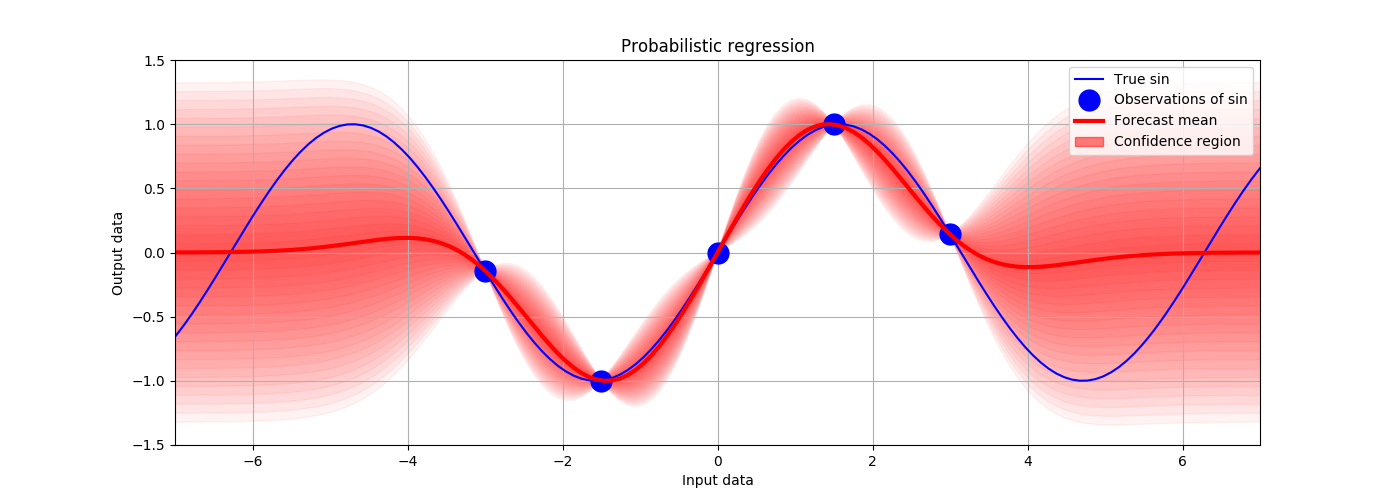
\includegraphics[scale=0.35]{images/probabilistic_regression}
\end{frame}

\begin{frame}
  \frametitle{Concrete Models}
  \begin{itemize}
  \item Bayesian Neural Networks
  \end{itemize}
  \begin{center}
    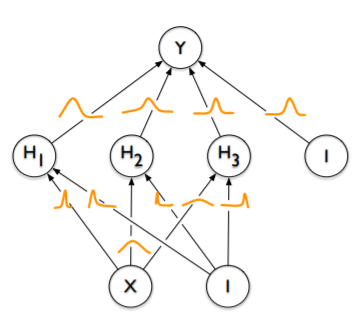
\includegraphics[scale=0.5]{images/bnn}
  \end{center}
\end{frame}

\begin{frame}
  \frametitle{Concrete Models}
  
  \begin{itemize}
  \item Mixture Density Networks
  \end{itemize}

  \begin{center}
    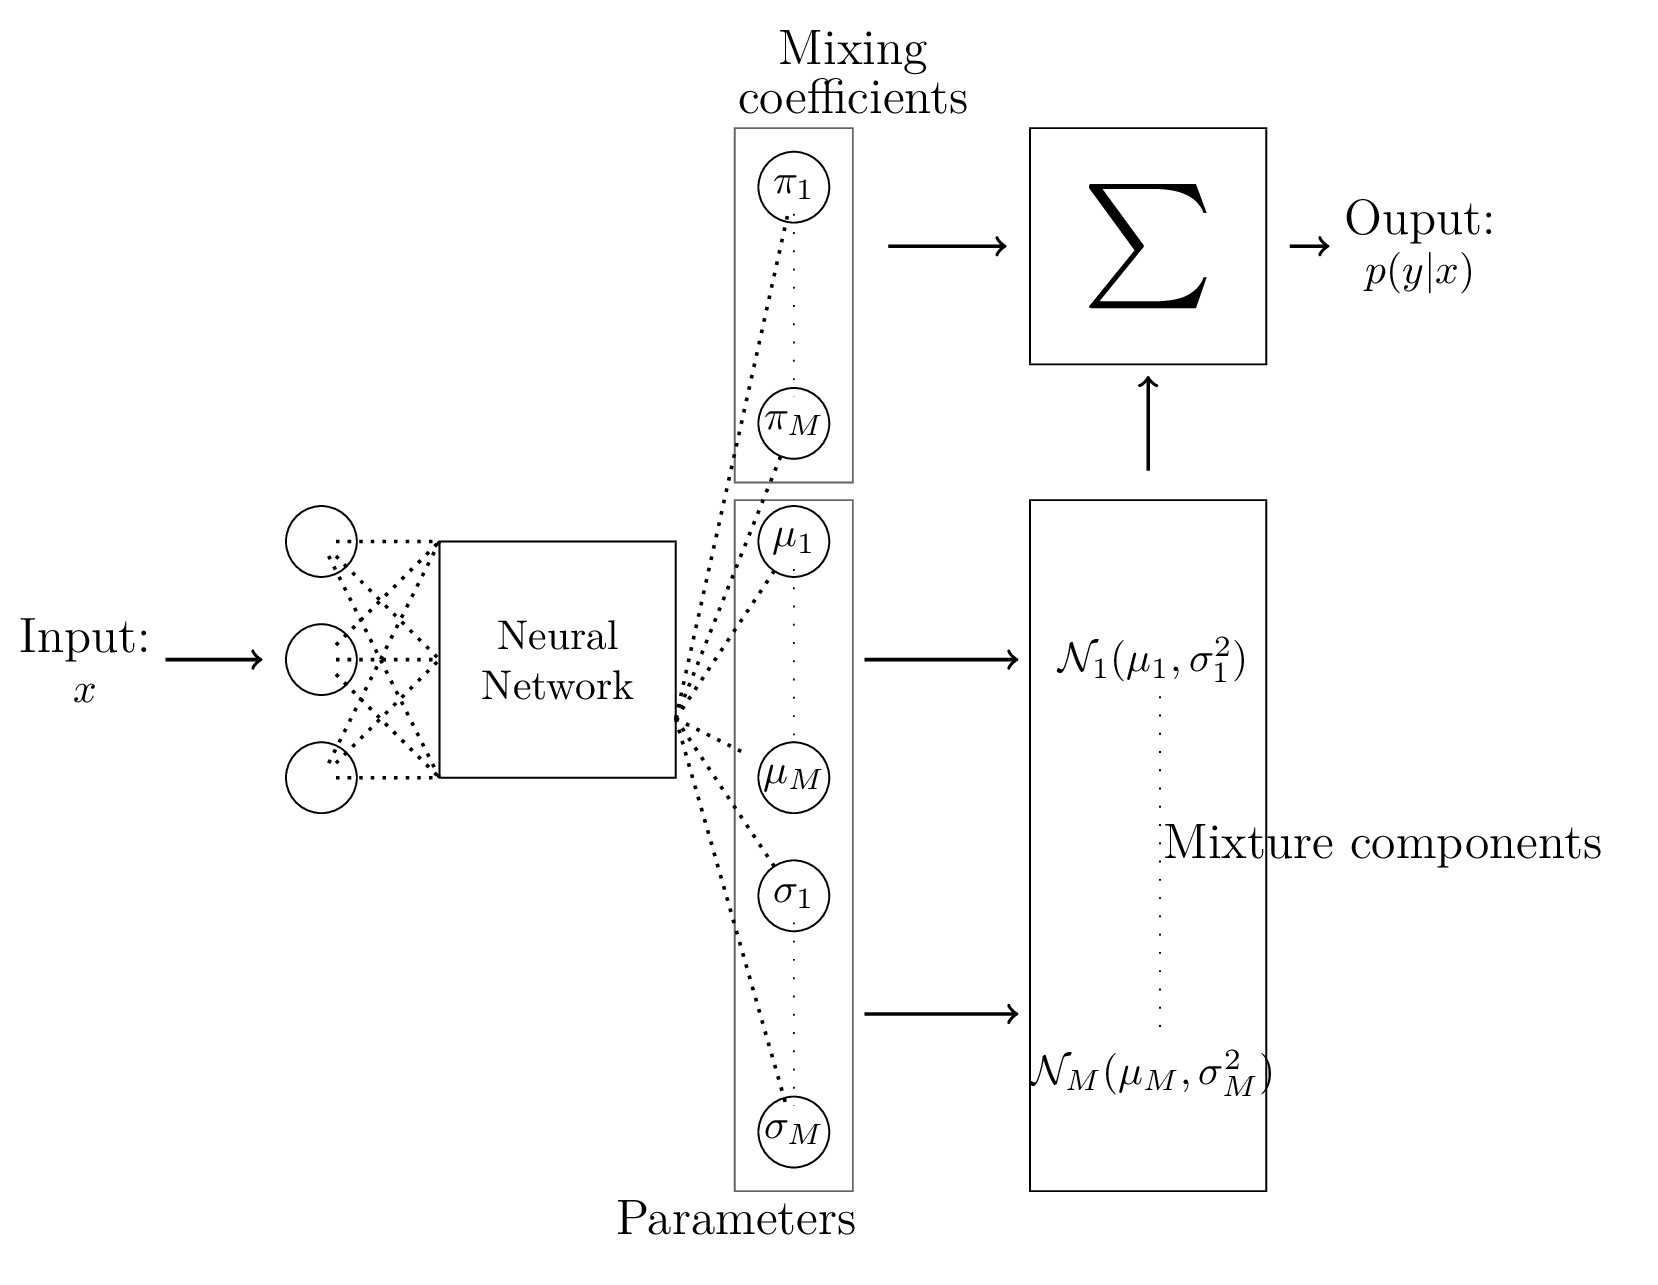
\includegraphics[scale=0.15]{images/mdn}
  \end{center}
  
\end{frame}

\begin{frame}[t]
  \frametitle{Concrete Models}
  Empirical model
  \begin{itemize}
  \item Past observations are treated as values of a random variable. From that a distribution for a predicted future value is implied.
  \item We use this model as a baseline.
  \end{itemize}
  We hope to achieve better results than the empirical model with the other two models.

\end{frame}

\begin{frame}
  \frametitle{Evaluation of probability distributions}
  \begin{itemize}
  \item We do not compare point estimate with a realized real value but rather a probability distribution with a real value.
  \end{itemize}
  \begin{center}
    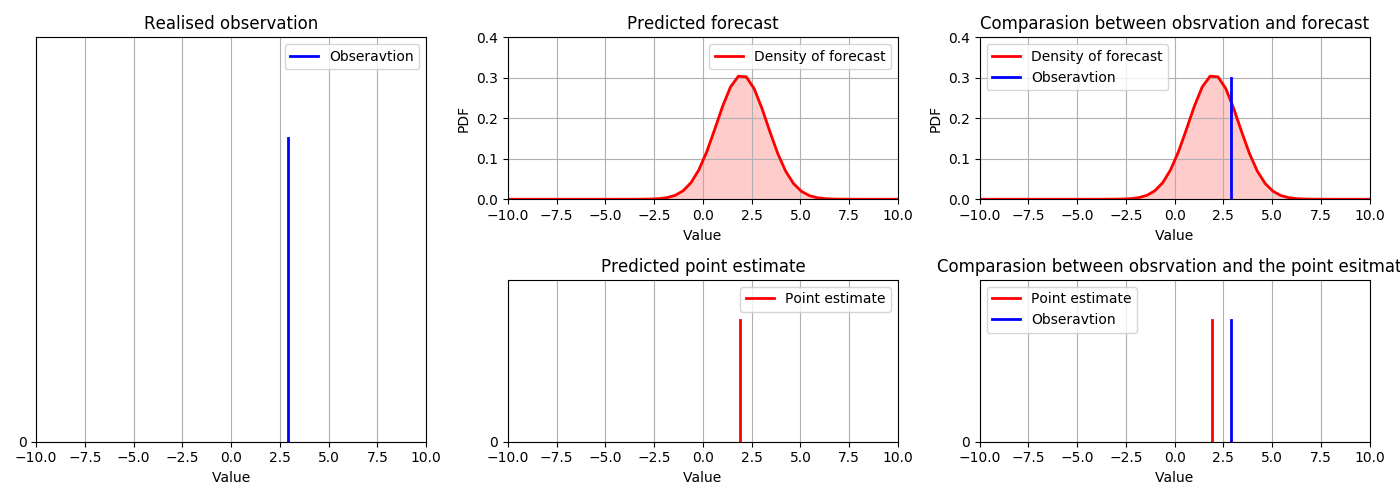
\includegraphics[width=.99\textwidth, height=0.5\textwidth]{images/distribution_point}
  \end{center}
\end{frame}

\begin{frame}
  \frametitle{Proper Scoring Rules}

  Continuous Rank Probability Score
  \begin{itemize}
  \item CRPS compares a distribution with an observation, where both are represented as cumulative distribution functions.
    $$  CRPS(F,y)  = \int_{-\infty}^{\infty}(F(x) - \mathbbm{1}\{y \leq x \})^2dx $$
  \end{itemize}
  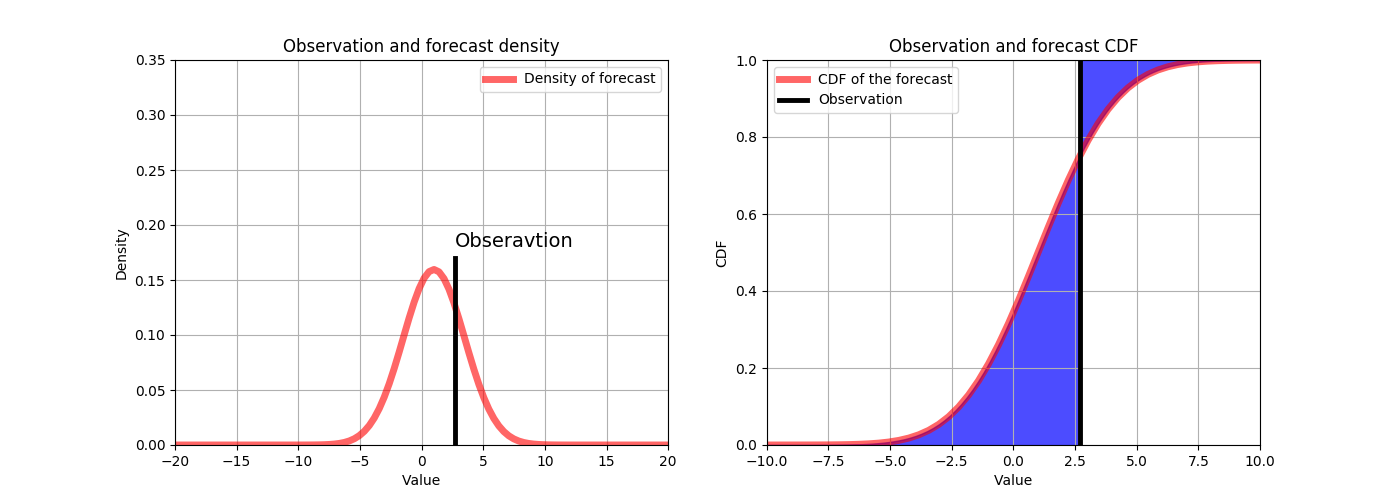
\includegraphics[scale=0.35]{images/crps}
\end{frame}

\begin{frame}[t]
  \frametitle{Verification Rank  Histograms}
  \begin{columns}
    \begin{column}[b]{0.3\textwidth}
      \begin{itemize}
      \item Does the observation behave like a random sample from the forecast distribution?
      \end{itemize}
    \end{column}
    \begin{column}{0.7\textwidth}
      \begin{center}
        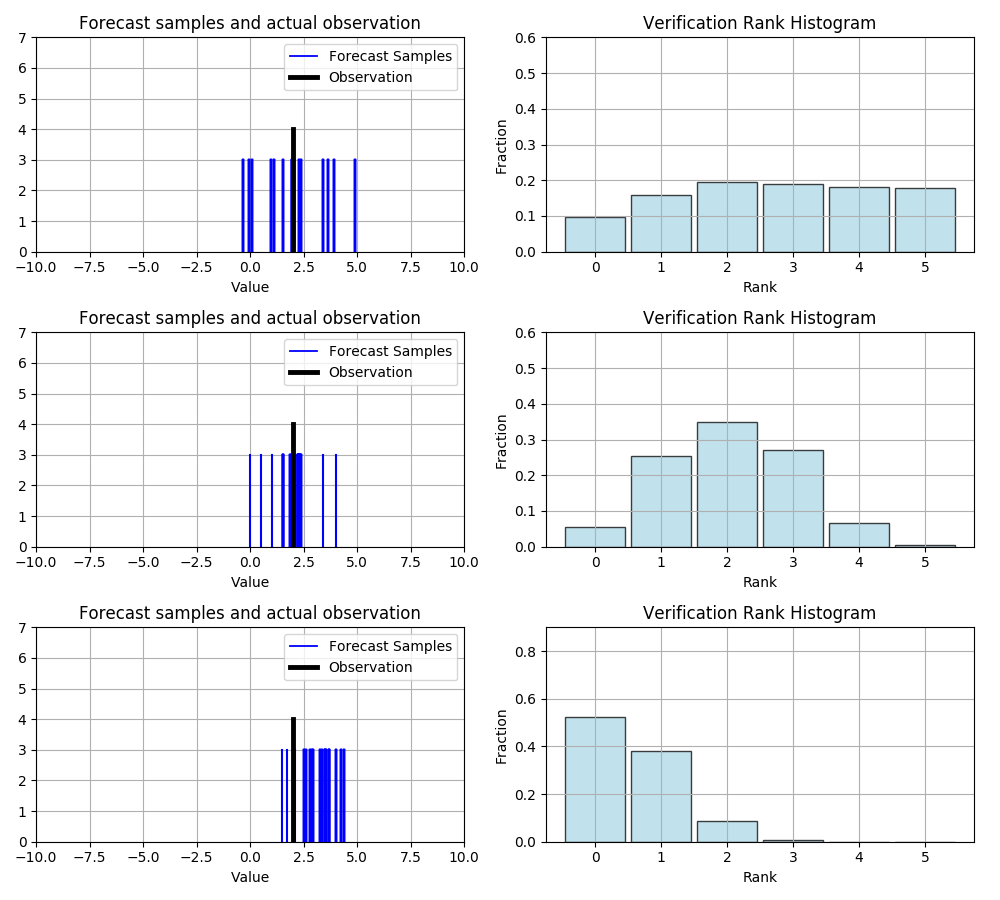
\includegraphics[scale=0.3]{images/verification_histogram}
      \end{center}
    \end{column}
  \end{columns}
\end{frame}

\begin{frame}
  \frametitle{Feature importance}
  \begin{itemize}
  \item Assess the \textbf{relative} importance of all features used by a model.
    \begin{itemize}
    \item \textcolor{red}{Important}: Importance is relative only to the model itself.
    \end{itemize}
    \item Random shuffling of each predictor/feature in the test set one at a time and observing the increase/decrease in mean the CRPS value compared to the unpermuted features.
  \end{itemize}
\end{frame}

\begin{frame}
  \frametitle{Training}
  \begin{itemize}
  \item Approach \\
    Based on the data and the examined types of models there are several orthogonal considerations to make when it comes to training:
    \begin{itemize}
    \item Target LUBW-Station -- SAKP, SBC, SNTR
    \item Integration period -- one day, twelve hours, one hour
    \item Use of the other two LUBW station -- yes or no
    \item Predicted air pollution value -- PM10 or PM2.5
    \item Used model - BNN or MDN (two types of MDNs)
    \end{itemize}
    We wanted to investigate every possible combination.
  \item Challenges:
    \begin{itemize}
    \item BNNs are very hard to train.
    \item A lot of possible ways to train several different models.
    \end{itemize}
  \end{itemize}
\end{frame}


\begin{frame}[t]
  \frametitle{Results}
  Results presented here: representative sample of all results.
  \pause
  \begin{itemize}
  \item Plots showing how exactly the built models predict the values of their train and test sets.
  \end{itemize}
\end{frame}

\begin{frame}[t]
  \frametitle{Results}
  Empirical Model, twelve hour averaged data
  \begin{center}
    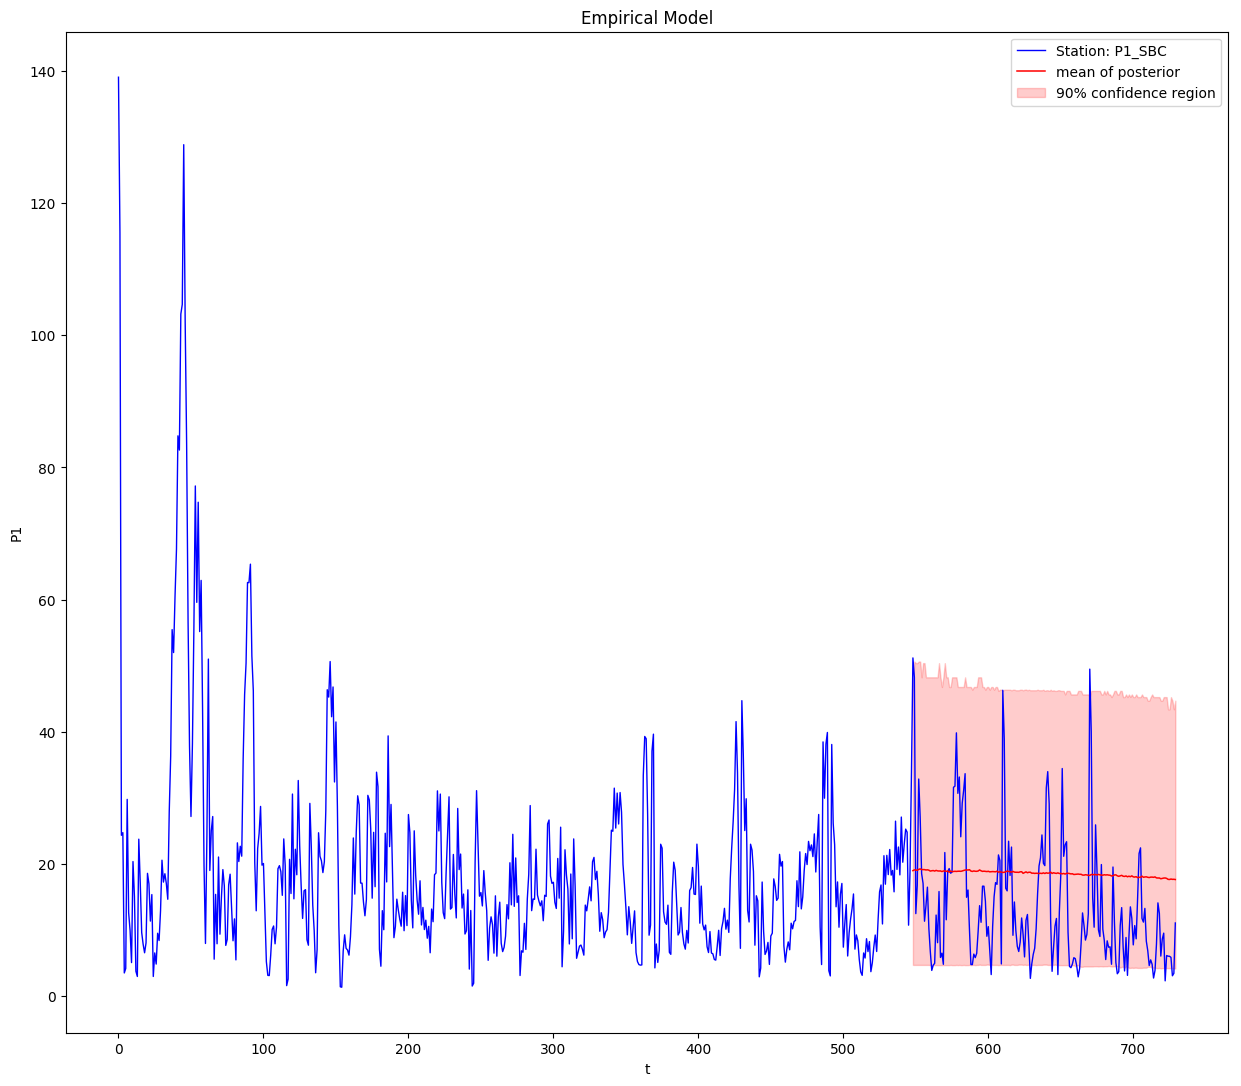
\includegraphics[scale=0.25]{images/12h/emp-12h}
  \end{center}  
\end{frame}

\begin{frame}[t]
  \frametitle{Results}
  MDN, twelve hour averaged data
  \begin{center}
    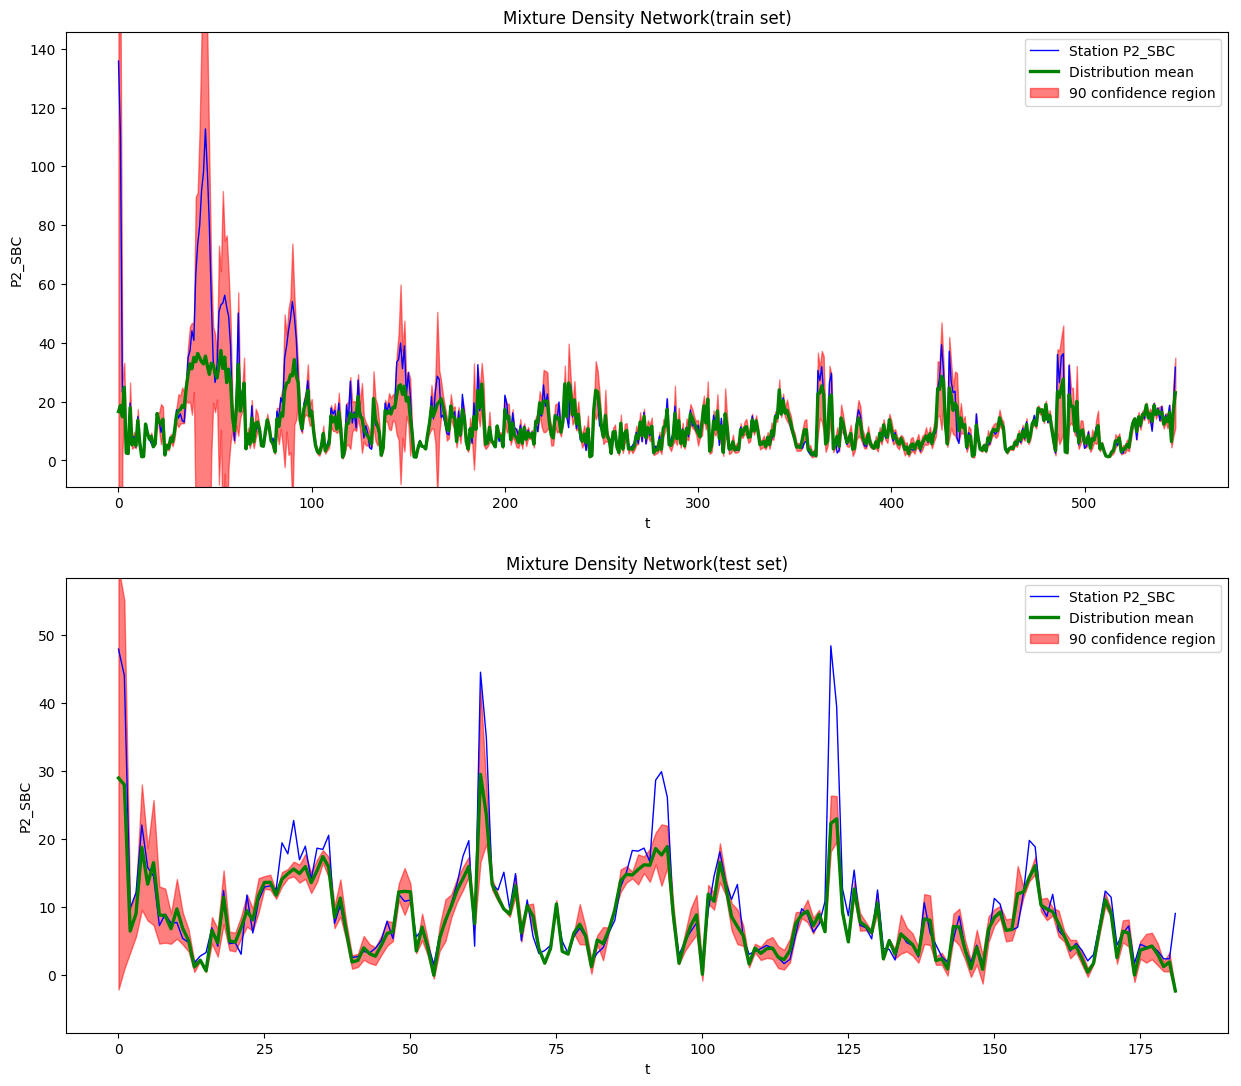
\includegraphics[scale=0.25]{images/12h/mdn_12h}
  \end{center}  
\end{frame}

\begin{frame}[t]
  \frametitle{Results}
  BNN, twelve hour averaged data
  \begin{center}
    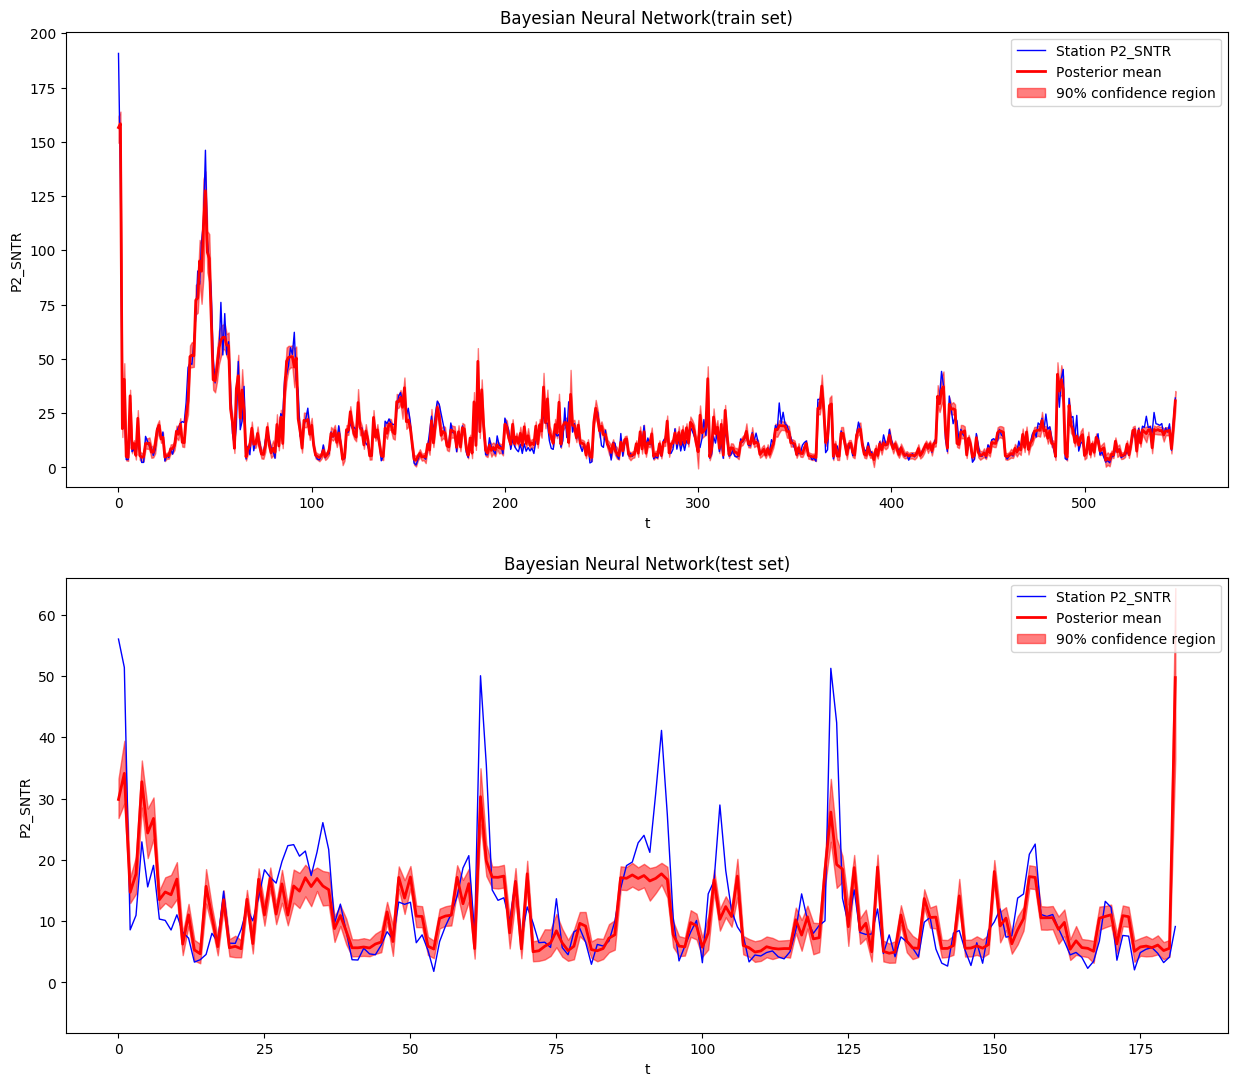
\includegraphics[scale=0.25]{images/12h/bnn_12h}
  \end{center}
\end{frame}

\begin{frame}[t]
  \frametitle{Results}
  Results presented here: representative sample of all results.
  \begin{itemize}
  \item Plots of the models modeling their respective test and train sets.
    \pause
  \item Plots comparing the built models with respect their CRPS score across LUBW Station, use of LUBW data and predicted air pollution value.
  \end{itemize}
\end{frame}

\begin{frame}[t]
  % \frametitle{Results}
  \begin{center}
    \vspace*{-0.2in}
    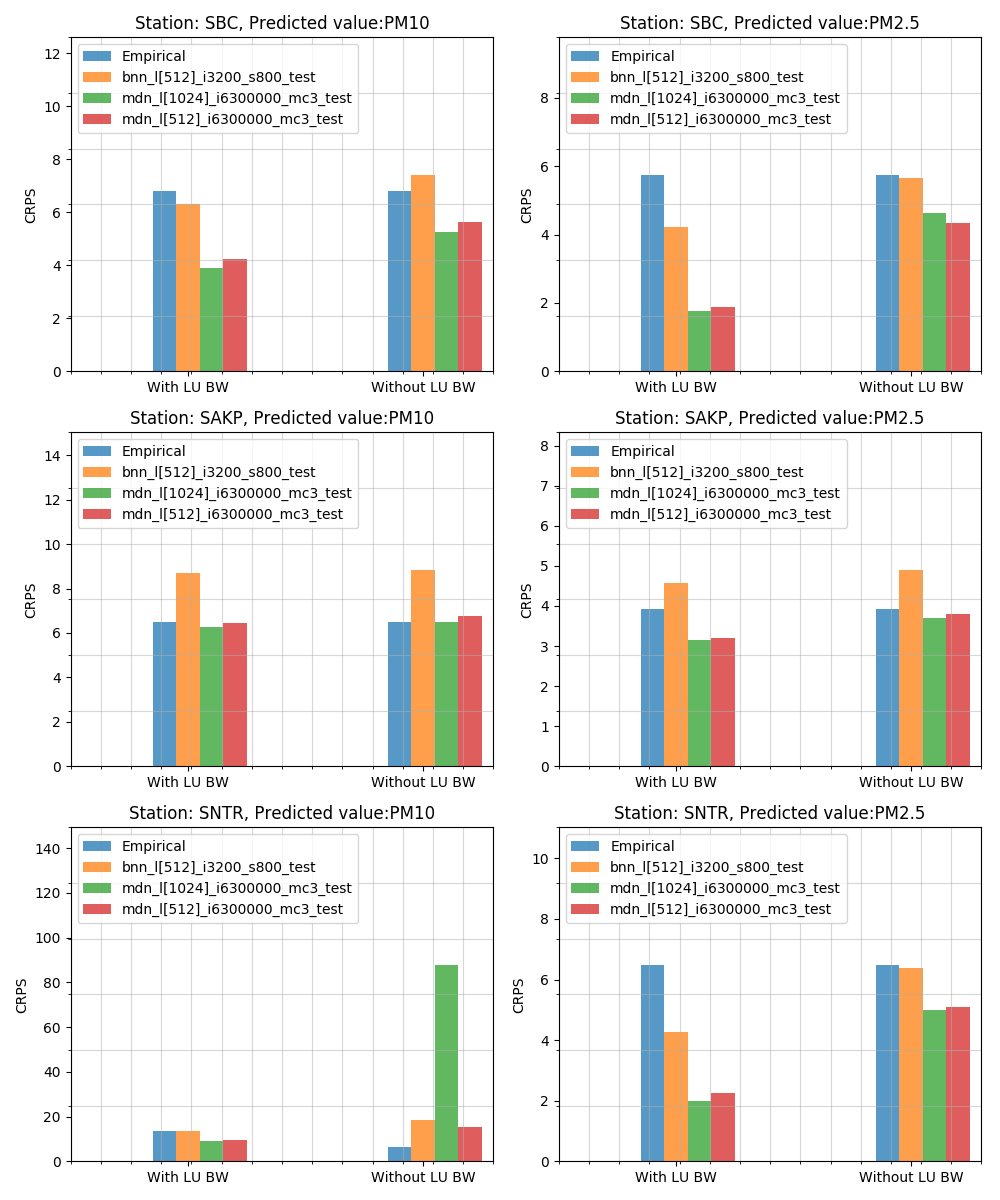
\includegraphics[height=0.75\textwidth, width=0.8\textwidth ]{images/1h/results_plot_CRPS}
  \end{center}
\end{frame}


\begin{frame}[t]
  \frametitle{Results}
  \begin{center}
    \vspace*{-0.2in}
    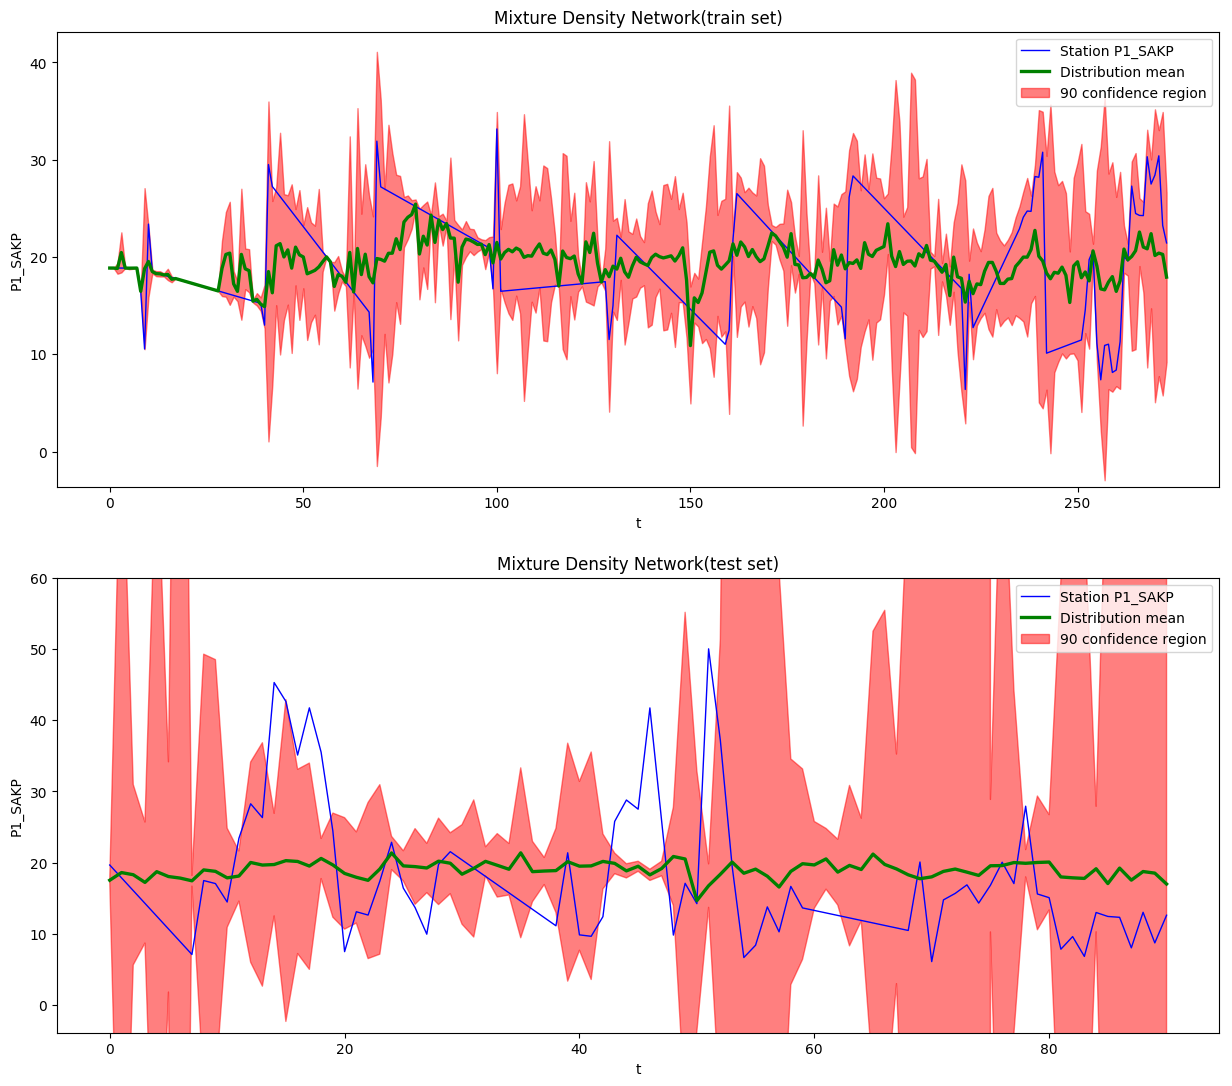
\includegraphics[height=0.65\textwidth, width=0.8\textwidth ]{images/mdn-bad}
  \end{center}
\end{frame}


\begin{frame}[t]
  \frametitle{Results}
  Results presented here: representative sample of all results.
  \begin{itemize}
  \item Plots of the models modeling their respective test and train sets.
  \item Plots comparing the built models with respect their CRPS score across LUBW Station, use of LUBW data and predicted air pollution value.
    \pause
  \item Two rank histograms reflecting the results of all built models.
  \end{itemize}
\end{frame}

\begin{frame}[t]
  \frametitle{Results}
  BNN (one day average) and MDN (one hour average), Rank Histograms  
  \begin{center}
    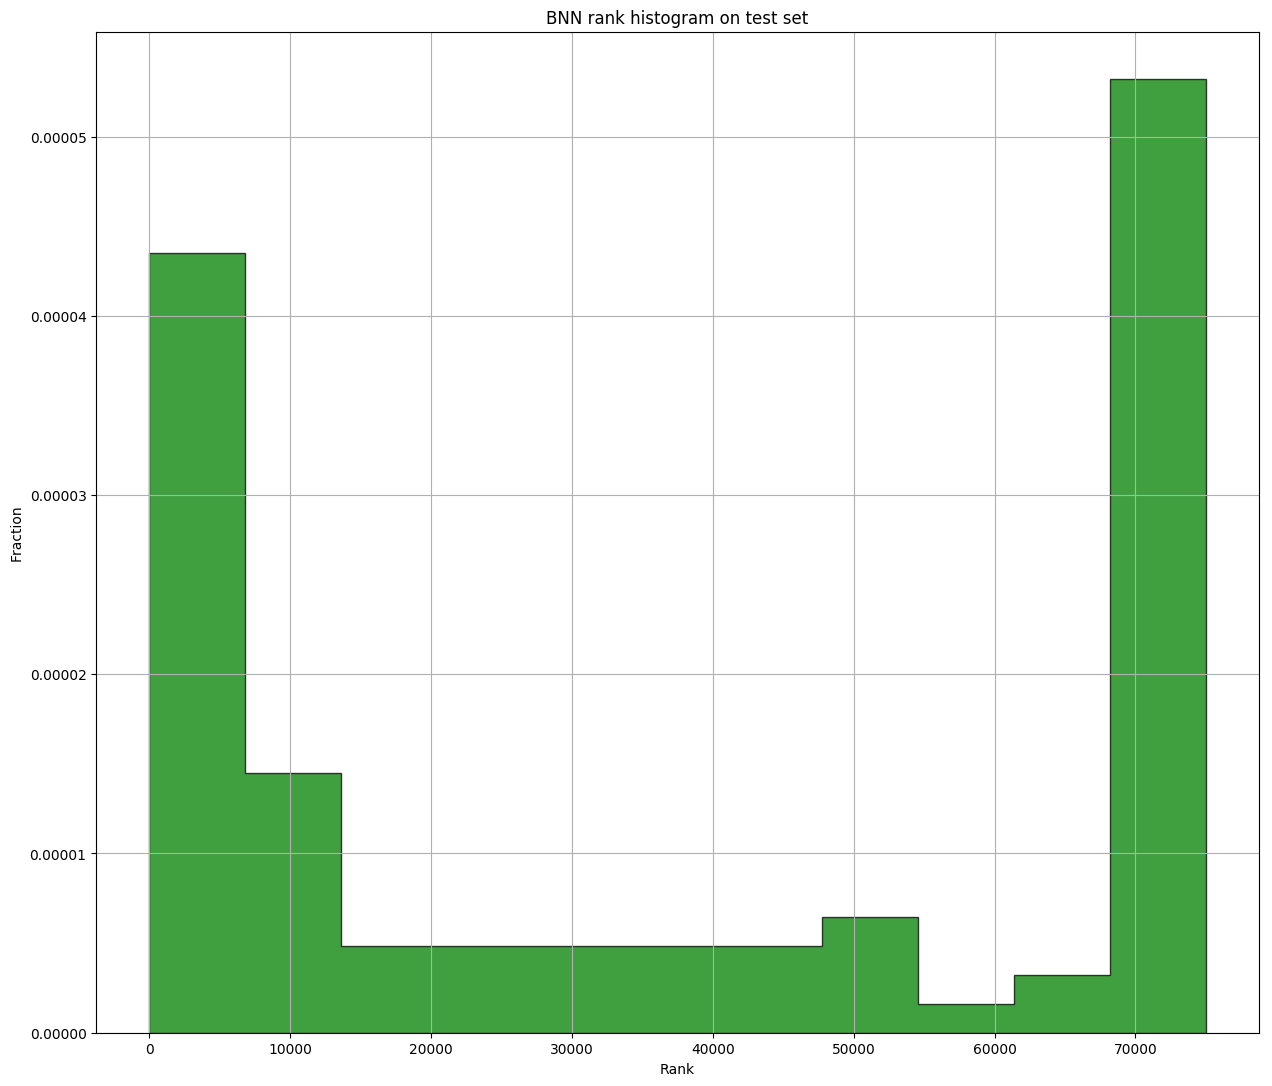
\includegraphics[height=0.45\textwidth, width=0.45\textwidth ]{images/ver/bnn-rank-1d}
    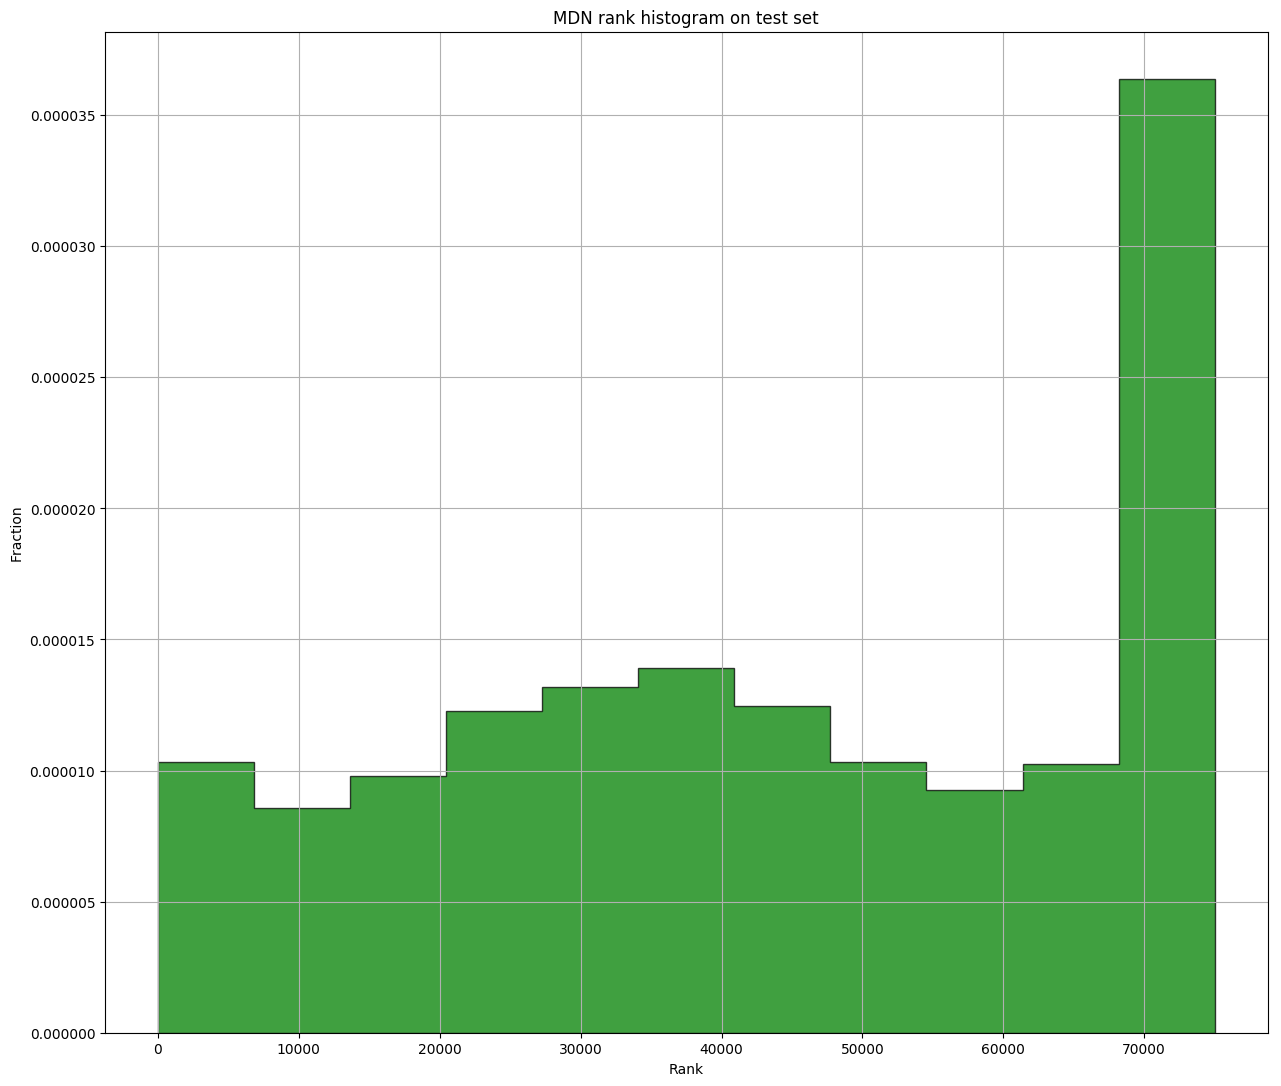
\includegraphics[height=0.45\textwidth, width=0.45\textwidth ]{images/ver/mdn-rank-1h}
  \end{center}  
\end{frame}


\begin{frame}[t]
  \frametitle{Results}
  Results presented here: representative sample of all results.
  \begin{itemize}
  \item Plots of the models modeling their respective test and train sets.
  \item Plots comparing the built models with respect their CRPS score across LUBW Station, use of LUBW data and predicted air pollution value.
  \item Two rank histograms reflecting the results of all built models.
    \pause
  \item Feature importance data.
  \end{itemize}
\end{frame}


\begin{frame}
  \vspace*{-0.05in}
  \begin{center}
    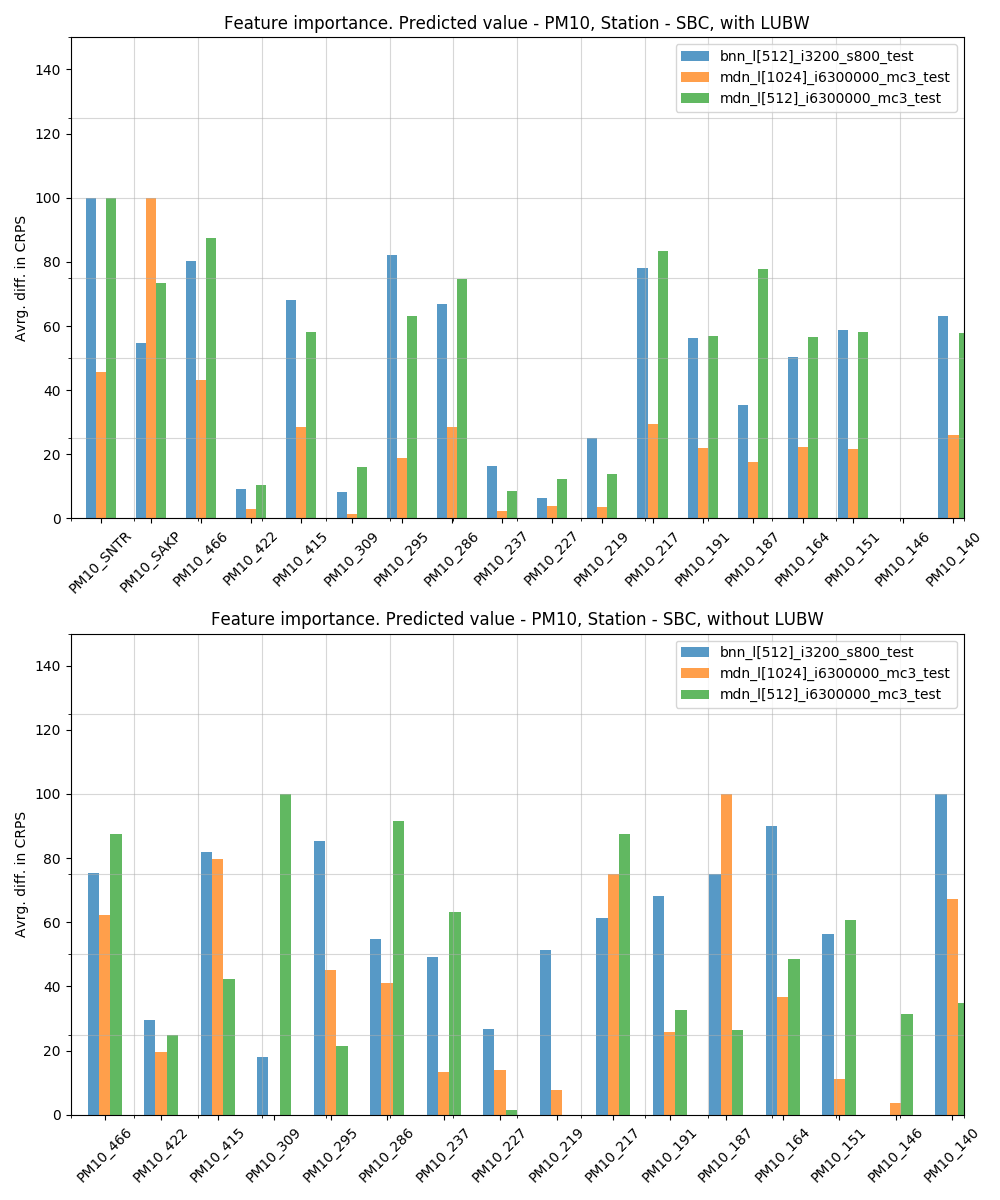
\includegraphics[height=0.75\textwidth, width=0.76\textwidth]{images/feature_importance_CRPS_SBC_P1}
  \end{center}  
\end{frame}


\begin{frame}[t]
  \frametitle[Short]{Conclusion}
  The results show:
  \begin{itemize}
  \item Stochastic regression models are a viable approach for predicting values in the investigated sensor network.
  \item Few sensors have consistently low feature importance for the built models.
  \item There is clearly room for improvement of the models.
  \end{itemize}
  
\end{frame}


\begin{frame}
  \frametitle{}
  \begin{center}
    \huge{Thank you for your attention.}    
  \end{center}
\end{frame}

\begin{frame}
  \frametitle{}
  \begin{center}
    \huge{Questions?}    
  \end{center}
\end{frame}

\end{document}

%%% Local Variables:
%%% mode: latex
%%% TeX-master: t
%%% End:
